% =====================================================================
% Ihara--Bass, the companion "Ihara side" to "Random Signs into Matchings"
% (Godsil--Gutman, Paper I) and "Unfolding a Graph into a Tree"
% (Heilmann--Lieb, Paper II). Same house style as Paper II: technical,
% unambiguous, story-driven (each section opens with a question), key formulas
% framed and centred, humility throughout. Honesty rules verbatim: "proven" =
% sorry-free; scope stated exactly; nothing hidden.
% Verified against the Lean source 2026-06-06 (lake build Ihara.Bass, exit 0;
% #print axioms SimpleGraph.bass_determinant -> propext, Classical.choice,
% Quot.sound only). Toolchain v4.30.0-rc2, local Mathlib.
% =====================================================================
\documentclass[11pt]{article}
\usepackage[T1]{fontenc}
\usepackage{lmodern}
\usepackage{amsmath,amssymb,amsthm,booktabs,graphicx,hyperref}
\usepackage{xurl}
\usepackage[table]{xcolor}
\definecolor{ggteal}{HTML}{1B6F8C}
\definecolor{ggband}{HTML}{DCE7EB}
\definecolor{ggamber}{HTML}{E08A1E}
\usepackage[margin=1in]{geometry}
\usepackage{microtype}
\usepackage[most]{tcolorbox}
\setlength{\emergencystretch}{2em}
\graphicspath{{figures/}}
\newtheorem{theorem}{Theorem}
\newtheorem{lemma}{Lemma}
\newtheorem{definition}{Definition}
\newcommand{\lean}[1]{\texttt{#1}}
\newcommand{\Z}{\mathbb{Z}}
\newcommand{\R}{\mathbb{R}}
\DeclareMathOperator{\Dart}{Dart}
\hypersetup{colorlinks=true,linkcolor=ggteal,citecolor=ggteal,urlcolor=ggteal}
% framed, centred display for the load-bearing formulas
\newtcbox{\keybox}{on line,boxrule=0.9pt,colframe=ggteal,colback=ggband!40,
  arc=3pt,left=8pt,right=8pt,top=5pt,bottom=5pt}
\newcommand{\keyeq}[1]{\begin{center}\keybox{$\displaystyle #1$}\end{center}}

\title{\bf Folding Edges into Vertices\\[4pt]
  \large\normalfont A machine-checked proof of Bass's determinant formula for the Ihara zeta in Lean~4}
\author{Carles Mar\'in\thanks{Formalized with AI assistance (Claude, Anthropic); the mathematics and all claims are the author's responsibility. The methodology is discussed in Section~\ref{sec:implications}.}\\[3pt]
  \normalsize Independent researcher\\
  \normalsize \texttt{karlesmarin@gmail.com}}
\date{June 2026}

\begin{document}
\maketitle

\begin{abstract}
This is a companion to \emph{Random Signs into Matchings}~\cite{PartI} and \emph{Unfolding a
Graph into a Tree}~\cite{PartII}, where I formalized the matching polynomial of a graph---the
\emph{tree} side of a walk count. Here I build the \emph{cycle} side: a machine-checked,
\lean{sorry}-free proof, in Lean~4 / Mathlib, of \emph{Bass's determinant formula} for the Ihara
zeta function. The reciprocal of the zeta function is $\det(I-uB)$, where $B$ is Hashimoto's
\emph{non-backtracking} operator on the $2|E|$ oriented edges; Bass's theorem collapses that
$2|E|$-dimensional determinant to an $|V|$-dimensional one built from the adjacency and degree
matrices. Along the way I formalize the non-backtracking operator, the oriented-edge incidence
calculus, and the determinant $\det(I+uJ)=(1-u^2)^{|E|}$ of the reversal involution, for none of
which could I find a prior formalization in any proof assistant. The headline theorem depends only
on the three standard axioms. I am exact about the boundary: I prove the identity over a field (the
standard setting; the proof inverts $I+uJ$, a unit exactly when $1-u^2\neq0$), the analytic zeta
function---the Euler product over prime cycles---is \emph{not} formalized, and full ring-generality
is mapped, not built. None of this is new mathematics; the contribution is the formalization, and
the fact that the cycle side of the matching/Ihara trace formula now stands beside the tree side in
the same library.
\end{abstract}

\noindent\emph{Reader's map.} If you read only one thing, read Theorem~\ref{thm:bass} and
Figure~\ref{fig:nb}---the identity, and the picture of why an edge-sized determinant is really a
vertex-sized one. The proof is a single journey: a four-identity incidence calculus
(Section~\ref{sec:proof}), the determinant of the reversal involution
$\det(I+uJ)=(1-u^2)^{|E|}$ obtained by orienting the edges (Figure~\ref{fig:reindex}), and a
Sylvester step that factors $I+uJ$ out and slides the incidence matrices past each other. The
load-bearing formulas are framed; the honest limits---the field hypothesis above all---are stated
as plainly as the result.

% ---------------------------------------------------------------
\section{Introduction: a short history, and why this paper}
\label{sec:intro}

\emph{Could a zeta function born in 1966 in the arithmetic of $p$-adic groups, quietly rediscovered
to be a statement about graphs, and turned in the 2010s into a workhorse of network science, be
placed beyond doubt by a machine---and what would that be good for?} Answering it requires several
threads of history to meet.

The first thread is \emph{number theory}. In 1966 Ihara~\cite{Ihara1966} attached a zeta function
to a discrete subgroup of $\mathrm{PGL}_2$ over a $p$-adic field, as a graph-free analogue of the
Selberg zeta function. Serre observed that Ihara's object was secretly combinatorial: the $p$-adic
group acts on a tree---its Bruhat--Tits tree---and the zeta depends only on the finite quotient
\emph{graph}. Stripped of its arithmetic origins, the \emph{Ihara zeta function} of a finite graph
$G$ counts its \emph{prime cycles}---classes of closed walks that never backtrack and are not powers
of shorter ones---through an Euler product $\zeta_G(u)=\prod_{[C]}(1-u^{\ell(C)})^{-1}$. A theorem
of number theory had become a theorem of graphs (Figure~\ref{fig:prime}).

\begin{figure}[t]
  \centering
  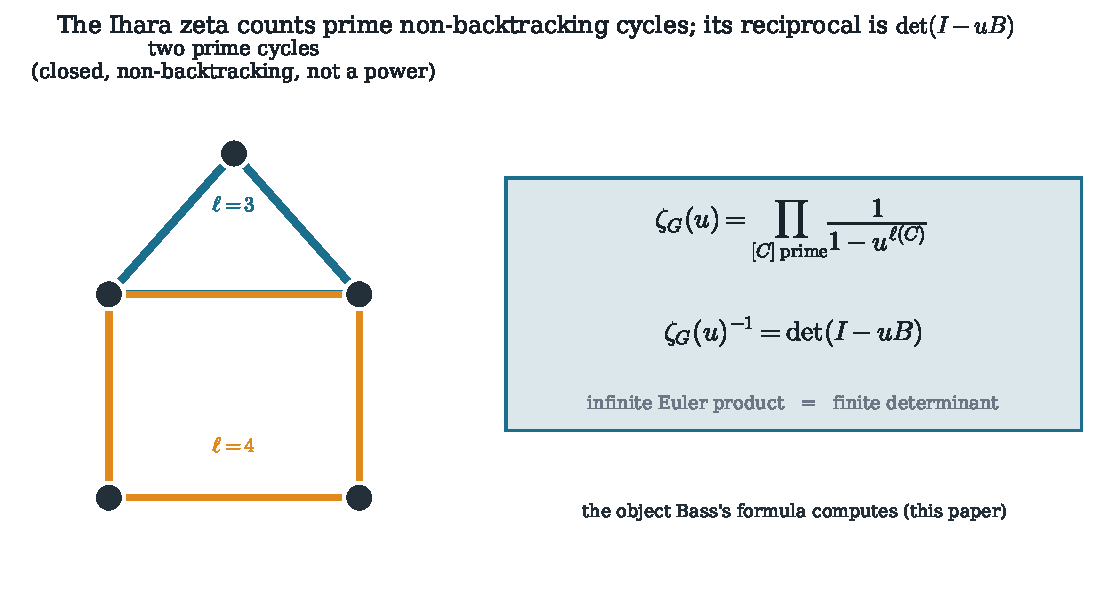
\includegraphics[width=\textwidth]{bass_fig4_primecycles.pdf}
  \caption{What the Ihara zeta counts. A graph's \emph{prime cycles} are its closed,
  non-backtracking walks that are not powers of shorter ones (two shown, of lengths $3$ and $4$).
  The zeta is their Euler product; its reciprocal is the finite determinant $\det(I-uB)$---the
  object Bass's formula computes, and this paper formalizes.}
  \label{fig:prime}
\end{figure}

The second thread is \emph{graph theory}. Sunada and then Hashimoto~\cite{Hashimoto1989} recast the
zeta function through a linear operator: the \emph{non-backtracking} (edge-adjacency) operator $B$
on the $2|E|$ oriented edges, with $\zeta_G(u)^{-1}=\det(I-uB)$. This is an honest determinant, but
a large one---its size is twice the number of edges. In 1992 Bass~\cite{Bass1992} proved the
identity that tames it, collapsing the $2|E|$-dimensional edge determinant to an $|V|$-dimensional
vertex determinant; Kotani--Sunada and Foata--Zeilberger later gave elementary
proofs~\cite{KotaniSunada2000}, and Terras's \emph{Stroll through the Garden}~\cite{Terras2011} is
the modern account. Bass's formula is the bridge between the combinatorial operator $B$ and the
spectral data $(A,D)$ a graph already wears on its sleeve.

The third thread ties this to the band of the earlier papers. A $d$-regular graph is
\emph{Ramanujan}---an optimal expander, its non-trivial spectrum inside
$[-2\sqrt{d-1},2\sqrt{d-1}]$---precisely when its Ihara zeta satisfies an analogue of the
\emph{Riemann hypothesis} (Sunada): the zeta's poles lie on a critical line, the multiplicative
image of the same band $2\sqrt{d-1}$ that confines the roots of the matching polynomial in
\emph{Unfolding a Graph into a Tree}~\cite{PartII}. The matching polynomial is the tree
(Plancherel) shadow of the walk count; the Ihara--Bass determinant is its cycle ($\pi_1$)
counterpart (Section~\ref{sec:trace}). And in the 2010s a fourth, applied thread arrived: the
largest non-backtracking eigenvalue sets the percolation and epidemic threshold of a network, and
the leading non-backtracking eigenvectors are a state-of-the-art tool for community
detection~\cite{KarrerNewmanZdeborova2014}. One operator $B$ runs through all four threads.

Against these stands the younger thread of \emph{formalization}. Systems such as Lean and its
library Mathlib now carry machine-checked proofs of substantial mathematics, yet neither the Ihara
zeta function, nor Bass's formula, nor even the non-backtracking operator appears to have been
formalized in any proof assistant. Papers~I and~II formalized the matching polynomial---the tree
side; \emph{this paper builds the cycle side.} The precise question it answers is:
\begin{quote}\itshape
  can the $2|E|$-dimensional non-backtracking determinant be computed, inside a proof assistant,
  from the $|V|$-dimensional adjacency and degree data---and certified?
\end{quote}
Why it matters is, again, the meeting of the threads: a verified Bass formula is the spectral
identity a network scientist's non-backtracking methods rest on, the combinatorial half of the
Ihara--zeta ``Riemann hypothesis'' for graphs, reusable edge-operator infrastructure for the
formal-mathematics community, and---with the tree side already in Lean---the missing endpoint of a
graph trace formula (Section~\ref{sec:trace}).

\begin{figure}[t]
  \centering
  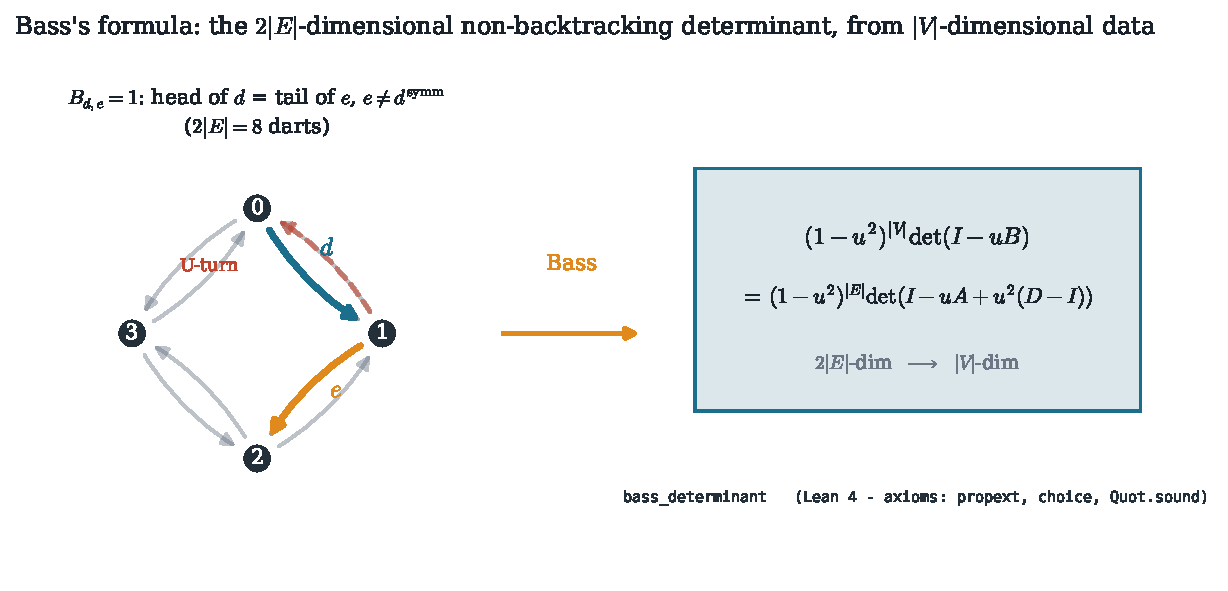
\includegraphics[width=\textwidth]{bass_fig1_nonbacktracking.pdf}
  \caption{Bass's formula on a small graph. The non-backtracking operator $B$ lives on the $2|E|$
  darts (left): $B_{d,e}=1$ when $d$'s head is $e$'s tail and $e$ is not $d$'s reverse (the U-turn,
  faded). Yet $\det(I-uB)$ is computable from the $|V|\times|V|$ adjacency/degree data (right).
  Machine-checked as \lean{bass\_determinant}.}
  \label{fig:nb}
\end{figure}

% ---------------------------------------------------------------
\section{The result}
\label{sec:result}

So much for the map; here is the territory. Write $A$ for the adjacency matrix, $D$ for the diagonal
degree matrix, and $B$ for Hashimoto's non-backtracking operator on the $2|E|$ oriented edges
(\emph{darts}). The reciprocal Ihara zeta is $\zeta_G(u)^{-1}=\det(I_{2|E|}-uB)$, and Bass's theorem
reduces it to vertex size.

\begin{theorem}[Bass's determinant formula, in Lean~4]
\label{thm:bass}
For a finite graph $G$ over a field, and $u$ in that field,
\keyeq{(1-u^2)^{|V|}\,\det\!\bigl(I-uB\bigr)\;=\;(1-u^2)^{|E|}\,\det\!\bigl(I-uA+u^2(D-I)\bigr).}
Equivalently $\det(I-uB)=(1-u^2)^{|E|-|V|}\det(I-uA+(D-I)u^2)$. The statement is \lean{sorry}-free;
\lean{\#print axioms SimpleGraph.bass\_determinant} reports only \lean{propext},
\lean{Classical.choice}, \lean{Quot.sound}.
\end{theorem}

Figure~\ref{fig:nb} shows the reduction; Table~\ref{tab:bass_results} lists every machine-checked
ingredient; Table~\ref{tab:bass_checks} confirms the identity numerically.

One feature of the statement repays a second look:
\begin{quote}\itshape
  why the prefactor $(1-u^2)^{|E|-|V|}$---why \emph{that} power, depending on nothing but the edge
  and vertex counts?
\end{quote}
Because the exponent is topological. For a connected graph $|E|-|V|=\beta_1-1$, where
$\beta_1=|E|-|V|+1$ is the \emph{first Betti number}---the number of independent cycles, the
dimension of the cycle space, the rank of $\pi_1(G)$. Bass's prefactor counts the graph's
independent loops; and it is exactly the multiplicity-$(|E|-|V|)$ pile-up of $\pm1$ eigenvalues of
$B$ that one sees in Figure~\ref{fig:spectrum}. A determinant identity quietly knows the topology of
the graph---which is, after all, only fair for the reciprocal of a function that counts its cycles.

\paragraph{The route, in one breath.}
Hashimoto's operator factors as $B=T^{\mathsf T}S-J$, where $S,T$ are the start/terminus incidence
matrices of the darts and $J$ is the reversal involution; so $I-uB=(I+uJ)-u\,T^{\mathsf T}S$. The
reversal involution has a clean determinant,
\keyeq{\det(I+uJ)\;=\;(1-u^2)^{|E|},}
because orienting each edge sorts the $2|E|$ darts into $|E|$ reversal pairs and turns $J$ into a
block diagonal of $2\times2$ swaps (Figure~\ref{fig:reindex}). Over a field with $1-u^2\neq0$, $I+uJ$
is then invertible; factoring it out of $I-uB$ and applying the Weinstein--Aronszajn identity to
slide $S$ past $T^{\mathsf T}$ delivers the $|V|$-dimensional determinant, and the incidence identity
$S(I-uJ)T^{\mathsf T}=A-uD$ identifies it as the right-hand side.

\paragraph{Contributions.} All in Lean~4 / Mathlib, all \lean{sorry}-free
(Table~\ref{tab:bass_results}):
\begin{enumerate}\itemsep2pt
\item \textbf{Bass's determinant formula} (\lean{bass\_determinant}) for every finite graph over a
  field, via the Sylvester reduction (Section~\ref{sec:proof}).
\item \textbf{The reversal-involution determinant} $\det(I+uJ)=(1-u^2)^{|E|}$
  (\lean{det\_one\_add\_smul\_reversal}), through an orientation reindex
  $\Dart\simeq\mathrm{Bool}\times\{\text{positive darts}\}$ (\lean{dartEquiv}) that
  block-diagonalizes $J$.
\item \textbf{Reusable infrastructure}: the non-backtracking operator on darts, the reversal
  involution, and the oriented-edge incidence calculus
  ($S T^{\mathsf T}=A$, $S S^{\mathsf T}=D=T T^{\mathsf T}$, $B=T^{\mathsf T}S-J$, $SJ=T$).
  Mathlib had none of these.
\end{enumerate}

\paragraph{What I claim as new.} The mathematics is classical (Section~\ref{sec:related}); the
novelty lies entirely in the formalization. I claim, specifically:
\begin{enumerate}\itemsep1.5pt
\item[(N1)] the first machine-checked proof I am aware of, in any proof assistant, of \emph{Bass's
  determinant formula}, and the first formalization of the non-backtracking (Hashimoto) operator and
  the Ihara-zeta reciprocal $\det(I-uB)$ (search-based; see the caveat below);
\item[(N2)] the orientation reindex \lean{dartEquiv} and the determinant
  $\det(I+uJ)=(1-u^2)^{|E|}$---a small, reusable piece of plumbing for any argument that must orient
  the edges of a graph;
\item[(N3)] the oriented-edge incidence calculus as named Lean lemmas, including a dart-counting
  lemma that realizes the adjacency matrix as $S T^{\mathsf T}$.
\end{enumerate}
None of (N1)--(N3) is new \emph{mathematics} in the theorem-proving sense; all are
\emph{formalization} contributions, and I separate them from the classical content deliberately.

\paragraph{And, plainly, what this is not.} It is a formalization of classical mathematics (Bass,
1992); it proves no new theorem and claims none. I prove the determinant identity, \emph{not} the
analytic Ihara zeta function (the Euler product over prime cycles is not formalized). I prove it
\emph{over a field}---the standard setting, and exactly what the Sylvester step needs, since it
inverts $I+uJ$, a unit only when $1-u^2\neq0$ (Section~\ref{sec:field}); full commutative-ring
generality is mapped, not built. And ``first formalization'' rests on a search of the three major
proof-assistant ecosystems---Lean/Mathlib, the Isabelle Archive of Formal Proofs, and
Coq/mathcomp---not a byte-level audit of every library, so I state it as exactly that.

% Tables for the Ihara–Bass formalization pearl.
% Requires \usepackage{booktabs,amsmath,amssymb} and \usepackage[table]{xcolor}
% in the main preamble, plus colors ggteal / ggband defined there.

% ---------- Table 1: formalised results ----------
\begin{table}[t]
  \centering
  \small
  \arrayrulecolor{ggteal}
  \caption{The formalised results (Lean~4 / Mathlib). All theorems are
  \texttt{sorry}-free; \texttt{\#print axioms} reports only \texttt{propext},
  \texttt{Classical.choice}, \texttt{Quot.sound}. The headline theorem is over a field
  (Section~\ref{sec:field}).}
  \label{tab:bass_results}
  \begin{tabular}{@{}llc@{}}
    \toprule
    \rowcolor{ggteal}
    \textcolor{white}{\textbf{Lean name}} & \textcolor{white}{\textbf{Statement}} & \textcolor{white}{\textbf{Status}} \\
    \midrule
    \rowcolor{ggband}
    \texttt{bass\_determinant} & $(1{-}u^2)^{|V|}\det(I{-}uB)=(1{-}u^2)^{|E|}\det(I{-}uA{+}u^2(D{-}I))$ & proven \\
    \texttt{det\_one\_add\_smul\_reversal} & $\det(I+uJ)=(1-u^2)^{|E|}$ & proven \\
    \rowcolor{ggband}
    \texttt{dartEquiv} & orientation reindex $\mathrm{Dart}\simeq\mathrm{Bool}\times\{\text{positive darts}\}$ & defined \\
    \texttt{hashimoto\_eq} & $B=T^{\mathsf T}S-J$ (non-backtracking $=$ follows $-$ reverses) & proven \\
    \rowcolor{ggband}
    \texttt{card\_posDart} & $|\{\text{positive darts}\}|=|E|$ (via the handshake lemma) & proven \\
    \texttt{startInc\_mul\_termInc\_transpose} & $S\,T^{\mathsf T}=A$ (darts realize the adjacency matrix) & proven \\
    \midrule
    \emph{analytic $\zeta_G$} & Euler product over prime cycles & future \\
    \rowcolor{ggband}
    \emph{$\mathrm{CommRing}$ generality} & universal-coefficient transfer from $\Z[u]$ & future \\
    \bottomrule
  \end{tabular}
  \arrayrulecolor{black}
\end{table}

% ---------- Table 2: numerical cross-checks ----------
\begin{table}[t]
  \centering
  \small
  \arrayrulecolor{ggteal}
  \caption{Numerical cross-checks of Bass's formula (SymPy, exact). For each graph the
  non-backtracking determinant $\det(I-uB)$ is computed directly on the $2|E|$ darts and matched
  against $(1-u^2)^{|E|-|V|}\det(I-uA+(D-I)u^2)$. Verified identically (also for $K_4$, where
  $|E|-|V|=2$, and the Petersen graph; polynomials omitted for length). The pendant vertices of the
  bull contribute trivial factors, so its determinant sees only the triangle.}
  \label{tab:bass_checks}
  \begin{tabular}{@{}lcclc@{}}
    \toprule
    \rowcolor{ggteal}
    \textcolor{white}{\textbf{$G$}} & \textcolor{white}{\textbf{$|V|$}} & \textcolor{white}{\textbf{$|E|$}} & \textcolor{white}{\textbf{$\det(I-uB)$}} & \textcolor{white}{\textbf{Bass?}} \\
    \midrule
    \rowcolor{ggband}
    $K_3$  & $3$ & $3$ & $(u^{3}-1)^{2}$ & $\checkmark$ \\
    $C_4$  & $4$ & $4$ & $(u^{4}-1)^{2}$ & $\checkmark$ \\
    \rowcolor{ggband}
    $C_5$  & $5$ & $5$ & $(u^{5}-1)^{2}$ & $\checkmark$ \\
    bull   & $5$ & $5$ & $(u^{3}-1)^{2}$ & $\checkmark$ \\
    \rowcolor{ggband}
    $K_4$  & $4$ & $6$ & degree $12$, $|E|-|V|=2$ (see source) & $\checkmark$ \\
    \bottomrule
  \end{tabular}
  \arrayrulecolor{black}
\end{table}


% ---------------------------------------------------------------
\section{What exactly are the objects?}
\label{sec:setting}

A question precedes the definitions:
\begin{quote}\itshape
  of all the operators one could hang on a graph's edges, why \emph{this} one---why forbid the
  single move of immediately turning back?
\end{quote}
Because backtracking floods a walk with trivial returns. On any graph the dominant contribution to
$\operatorname{tr}(A^k)$ comes from walks that wander out and retrace their steps---the very returns
a tree already has, the tree shadow of Section~\ref{sec:trace}. Strip the U-turns and only the
genuine cycle content survives: the non-backtracking operator's spectrum sees the graph's loops, not
its tree shadow, and its leading eigenvalue measures true branching. That is why the \emph{same}
operator that defines the Ihara zeta also sets a network's percolation threshold---both are asking,
at bottom, how fast non-retracing walks proliferate. With that motive in hand, the operators must be
pinned down. I work over a finite vertex
type $V$ with decidable adjacency. Mathlib already has the type \lean{SimpleGraph.Dart} of
\emph{oriented} edges; reversal $d\mapsto d^{\mathrm{symm}}$ is a fixed-point-free involution on the
$2|E|$ darts, and that involution is the whole reason the formula has the shape it does.

\begin{definition}[The four operators]
Over a commutative ring $R$: the \emph{degree matrix}
$D=\operatorname{diagonal}(v\mapsto\deg v)$; the \emph{reversal} permutation matrix $J$, with
$J_{d,e}=[\,e=d^{\mathrm{symm}}\,]$; the \emph{non-backtracking} (Hashimoto) operator $B$, with
$B_{d,e}=[\,d.\mathrm{snd}=e.\mathrm{fst}\ \wedge\ e\neq d^{\mathrm{symm}}\,]$; and the
start/terminus incidence matrices $S,T\colon V\times\Dart$, with $S_{v,d}=[\,d.\mathrm{fst}=v\,]$,
$T_{v,d}=[\,d.\mathrm{snd}=v\,]$.
\end{definition}

With $A$ Mathlib's adjacency matrix, the theorem proved is the framed identity of
Theorem~\ref{thm:bass}, stated in Lean over a field. Mathlib has a rich theory of simple graphs,
darts and determinants, but no non-backtracking operator and no Ihara zeta; building the operator
and its incidence calculus was a prerequisite, and I could find no prior formalization of Bass's
formula---or of the Hashimoto operator's determinant---in any proof assistant.\footnote{Best-effort
search across Lean/Mathlib, the Archive of Formal Proofs (Isabelle), and the Coq/MathComp ecosystem
(June~2026): graph adjacency, characteristic polynomials, and the matching polynomial (in my own
earlier work) appear, but I found no formalization of the Ihara zeta function, Bass's formula, or
the non-backtracking operator. Hence ``to my knowledge''.}

% ---------------------------------------------------------------
\section{How a machine reduces $2|E|$ to $|V|$}
\label{sec:proof}

Before any tactic, a question worth pausing on:
\begin{quote}\itshape
  why should a determinant over $2|E|$ edges be secretly a determinant over $|V|$ vertices at
  all---what makes the larger object collapse?
\end{quote}
The answer is hidden in the \emph{shape} of $B$, and it is the conceptual heart of the whole
formula. Hashimoto's operator is not arbitrary: it splits as $B=T^{\mathsf T}S-J$, a part
$T^{\mathsf T}S$ that \emph{factors through the vertices}---it has rank at most $|V|$, since $S$ and
$T$ both pass through the $|V|$-dimensional vertex space---plus the reversal involution $J$. The
vertex-factoring part is exactly what a Sylvester identity can push down to size $|V|$; the
involution $J$ is exactly what the powers of $(1-u^2)$ absorb. So the collapse is no miracle: it is
the statement that the edge operator carries only $|V|$ vertices' worth of genuine spectral
information, wrapped in an involution. Bass's formula is the precise bookkeeping of that split, and
the proof below is that bookkeeping made explicit. The classical argument factors the large
determinant by inverting $I+uJ$ and sliding the incidence matrices past one another; turning it into
a checked proof meant making each ``observe that'' explicit, in three movements.

\paragraph{The incidence calculus.}
Everything rests on four identities, each a finite sum over darts (all numerically pre-verified
before formalization):
\keyeq{S\,T^{\mathsf T}=A,\qquad S\,S^{\mathsf T}=D=T\,T^{\mathsf T},\qquad
  B=T^{\mathsf T}S-J,\qquad S\,J=T.}
The first says the darts from $v$ to $w$ realize the adjacency matrix (a dart-counting lemma,
\lean{adj\_dart\_card}); the third is the definition of ``non-backtracking'' as ``follows, minus
reverses''; the fourth says reversal swaps a dart's two ends. From $SJ=T$ together with $J^{\mathsf
T}=J$ and $J^2=I$ one then gets the companion $T\,T^{\mathsf T}=D$ for free, reusing $S\,S^{\mathsf
T}=D$ rather than re-counting.

\paragraph{The determinant of the reversal involution.}
The load-bearing computation is $\det(I+uJ)=(1-u^2)^{|E|}$. Here is the idea, and the one place a
real choice enters. Fix any linear order on $V$; call a dart \emph{positive} when its tail precedes
its head. Each edge has exactly one positive dart, and the reversal of a non-positive dart is
positive. This yields an equivalence (\lean{dartEquiv}, Figure~\ref{fig:reindex})
\keyeq{\Dart\;\simeq\;\mathrm{Bool}\times\{\text{positive darts}\},}
under which $J$---which merely swaps each dart with its reverse---becomes a \emph{block diagonal} of
the $2\times2$ swap, one block per edge. Hence $I+uJ$ becomes a block diagonal of
$\bigl(\begin{smallmatrix}1&u\\u&1\end{smallmatrix}\bigr)$, and since the positive darts biject with
the edges ($|\{\text{positive darts}\}|=|E|$, by the handshake lemma; \lean{card\_posDart}),
Mathlib's \lean{Matrix.det\_blockDiagonal} gives
$\det(I+uJ)=(1-u^2)^{|E|}$, each block contributing $1-u^2$.

\begin{figure}[t]
  \centering
  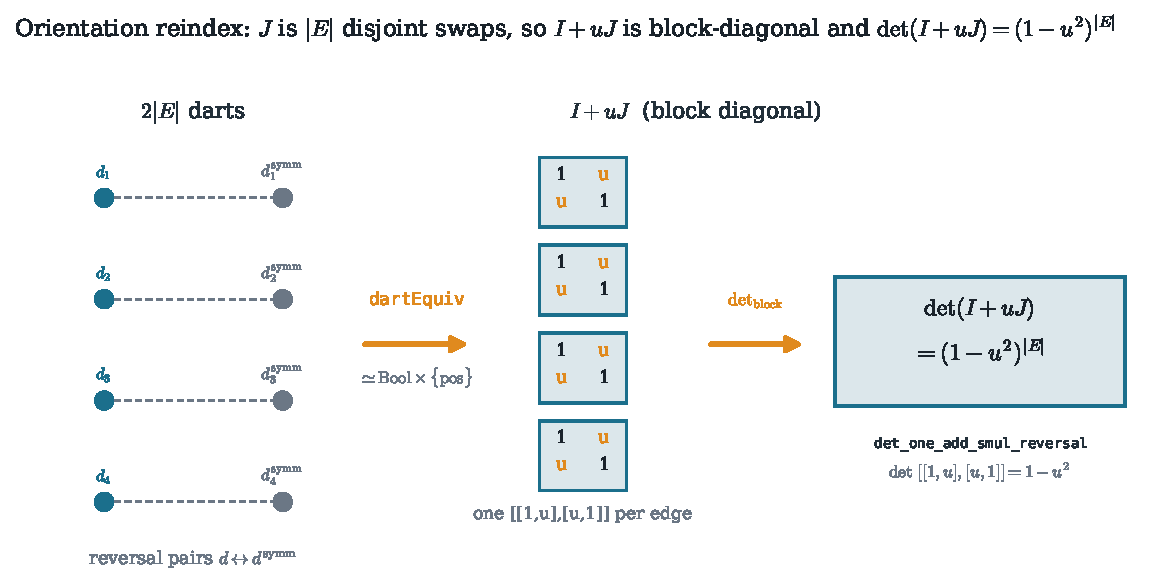
\includegraphics[width=\textwidth]{bass_fig2_reindex.pdf}
  \caption{The orientation reindex \lean{dartEquiv}: choosing a direction per edge sorts the $2|E|$
  darts into $|E|$ reversal pairs, block-diagonalizing $J$. Then $I+uJ$ is a block diagonal of
  $\bigl(\begin{smallmatrix}1&u\\u&1\end{smallmatrix}\bigr)$, so $\det(I+uJ)=(1-u^2)^{|E|}$
  (\lean{det\_one\_add\_smul\_reversal}).}
  \label{fig:reindex}
\end{figure}

\paragraph{The Sylvester reduction.}
Since $B=T^{\mathsf T}S-J$, we have $I-uB=(I+uJ)-u\,T^{\mathsf T}S$. Over a field with $1-u^2\neq0$,
the previous step makes $I+uJ$ \emph{invertible}, with $(I+uJ)^{-1}=(1-u^2)^{-1}(I-uJ)$ (immediate
from $(I+uJ)(I-uJ)=(1-u^2)I$). Factoring it out and applying the Weinstein--Aronszajn identity
\lean{Matrix.det\_one\_sub\_mul\_comm} to slide $S$ past $T^{\mathsf T}$ gives the
$|V|$-dimensional determinant
\[
  \det(I-uB)=(1-u^2)^{|E|}\det\!\bigl(I-u\,S(I+uJ)^{-1}T^{\mathsf T}\bigr),
\]
and the incidence identity $S(I-uJ)T^{\mathsf T}=A-uD$ collapses the right factor to
$(1-u^2)^{-|V|}\det(I-uA+u^2(D-I))$. Clearing denominators is the theorem. The degenerate value
$u^2=1$, where $I+uJ$ is singular, is handled separately: there the claim reduces to the no-edge and
empty-graph cases, where both sides vanish or are trivially equal.

% ---------------------------------------------------------------
\section{Where the field hypothesis comes from}
\label{sec:field}

It would be easy to state the theorem over an arbitrary commutative ring and quietly hope; I do not.
The Sylvester reduction \emph{inverts} $I+uJ$ and \emph{divides} by $1-u^2$, both legitimate only
when $1-u^2$ is a unit---i.e.\ over a field, away from $u^2=1$. This is the standard setting for
Bass's formula (one works over $\mathbb{C}$), and it is honest to say so rather than to dress the
proof in more generality than it has.

The reason the gap is real, not cosmetic: the inverse-free manipulations alone---multiply by
$I-uJ$, use $\det(I-uJ)=(1-u^2)^{|E|}$ and Weinstein--Aronszajn at $t=1$---deliver the identity
\emph{multiplied by an extra $(1-u^2)^{|E|}$}, and recovering the tight statement needs to cancel
that factor, which a field permits and a ring with zero-divisors does not. Full commutative-ring
generality nonetheless follows by a universal-coefficient transfer: prove the identity over
$\Z[u]$, where $1-u^2$ is a non-zero-divisor and the cancellation is legal, then base-change along
any ring map $\Z[u]\to R,\ u\mapsto u$, using that determinants commute with ring homomorphisms. I
describe this route but do not carry it out; the field version is what is machine-checked, and I
claim no more.

% ---------------------------------------------------------------
\section{Two sides of one trace formula}
\label{sec:trace}

What does the Ihara side have to do with the matching polynomial of
Papers~I and~II~\cite{PartI,PartII}? They are the two halves of a single accounting of
closed walks. Schematically, the trace of a power of the adjacency matrix splits into a
\emph{tree-like} part and a \emph{cyclic} part,
\keyeq{\operatorname{tr}(A^k)\;=\;\underbrace{p_k}_{\text{matching poly / tree}}
  \;+\;\underbrace{N_k}_{\text{non-backtracking / cycles}},}
with the same band $2\sqrt{\Delta-1}$ governing both sides (Figure~\ref{fig:trace}).

\begin{figure}[t]
  \centering
  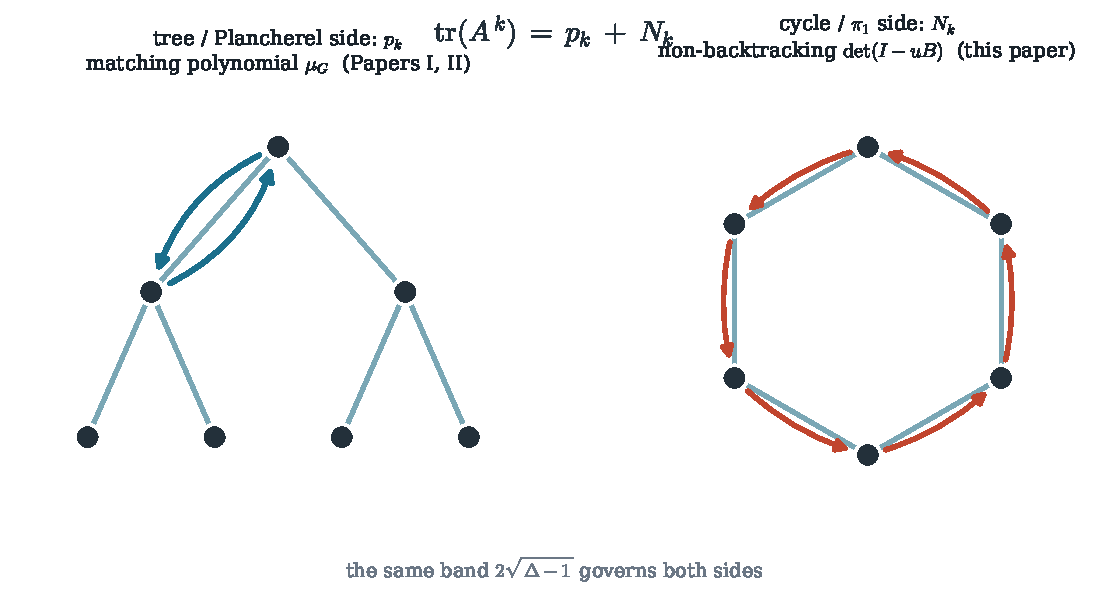
\includegraphics[width=0.92\textwidth]{bass_fig5_trace.pdf}
  \caption{Two sides of one accounting of closed walks. The tree (Plancherel) part $p_k$ is the
  matching polynomial---the walk count on the universal cover, where every return is a backtrack
  (Papers~I and~II); the cycle ($\pi_1$) part $N_k$ is the non-backtracking count $\det(I-uB)$ of
  this paper. The same band $2\sqrt{\Delta-1}$ confines both. With both endpoints now in Lean, the
  trace formula $p_k=\operatorname{tr}(A^k)-N_k$ becomes a well-posed next target.}
  \label{fig:trace}
\end{figure} The matching polynomial is the
universal-cover (tree) shadow of the walk count; the Ihara--Bass determinant counts the genuine
cycles, organized by the fundamental group $\pi_1$.

Here is a question worth carrying away from this paper:
\begin{quote}\itshape
  why should the \emph{same} number, $2\sqrt{\Delta-1}$, bound the roots of the matching polynomial
  (Paper~II) and mark the critical line of the Ihara zeta---two objects built from $G$ in seemingly
  unrelated ways?
\end{quote}
Because both are shadows of one object: the $\Delta$-regular tree that universally covers $G$. Its
spectral radius is exactly $2\sqrt{\Delta-1}$ (Kesten, 1959). The matching polynomial sees that
number as the edge of the tree's Plancherel (Kesten--McKay) measure; the Ihara zeta sees it as the
critical line of a Riemann hypothesis for graphs. One tree, two shadows, one number---and a reason
to suspect that the trace formula above is precisely the statement that makes the coincidence no
coincidence. With the tree side formalized in the earlier papers and the cycle side here, both
endpoints of that bridge now exist in Lean, and the trace formula itself
($p_k=\operatorname{tr}(A^k)-N_k$, sharp up to the girth) becomes a well-posed next target.

A first dividend is already visible. Bass's $(1-u^2)^{|E|-|V|}$ prefactor is exactly the source of a
striking feature of the non-backtracking spectrum: a multiplicity-$(|E|-|V|)$ pile-up of eigenvalues
at $\pm1$, with the remaining ``cycle'' eigenvalues filling a disk whose radius is set by the degree
variance, not the mean (Figure~\ref{fig:spectrum})---the same disk whose real edge gives the
percolation threshold.

\begin{figure}[t]
  \centering
  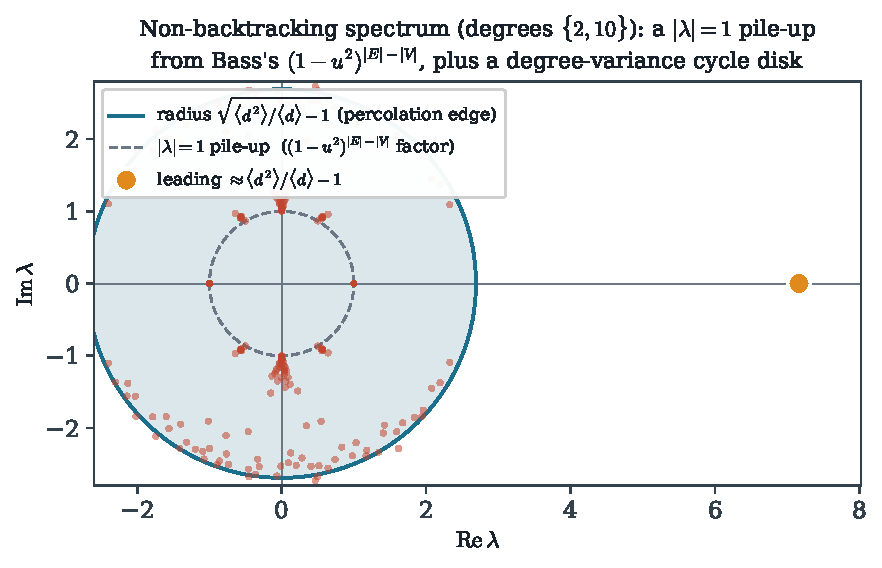
\includegraphics[width=0.9\textwidth]{bass_fig3_spectrum.pdf}
  \caption{The non-backtracking spectrum of a degree-irregular graph (configuration model, degrees
  $2$ and $10$). A large multiplicity sits on the unit circle---the $\pm1$ eigenvalues forced by
  Bass's $(1-u^2)^{|E|-|V|}$ factor---while the ``cycle'' eigenvalues fill a disk of radius
  $\sqrt{\langle d^2\rangle/\langle d\rangle-1}$ (degree-variance, not mean), whose real edge is the
  percolation threshold. Computed; the structure is explained by \lean{bass\_determinant}.}
  \label{fig:spectrum}
\end{figure}

% ---------------------------------------------------------------
\section{Implications}
\label{sec:implications}

Three kinds of implication, in decreasing order of how confidently I can claim them, and a
methodological aside.

\paragraph{Reusable, certified building blocks.}
The non-backtracking operator, the oriented-edge incidence calculus, the reversal-involution
determinant $\det(I+uJ)=(1-u^2)^{|E|}$, and the orientation reindex are now machine-checked and
available to anyone formalizing spectral graph theory, expander mixing, or zeta functions of graphs;
Mathlib had none of them. The reindex $\Dart\simeq\mathrm{Bool}\times\{\text{positive darts}\}$ in
particular is a small but genuinely reusable piece of plumbing for any argument that needs to orient
edges. This is the implication I can state most firmly.

\paragraph{A foothold for the trace formula and beyond.}
With both the matching-polynomial (tree) and Ihara--Bass (cycle) sides formalized, the graph trace
formula uniting them is now a concrete target, as is the analytic Ihara zeta---the prime-cycle Euler
product for which this determinant is the reciprocal. Should those landmarks be built, these are
foundations they can stand on.

\paragraph{The mathematics, with a note of caution.}
Non-backtracking spectra underpin sharp epidemic and percolation thresholds, spectral community
detection, and expander analysis---which is why the underlying identity matters. I am wary, though,
of borrowing that importance for this paper: formalizing a foundational determinant identity does
not by itself ship an algorithm or a network. Its value lies in certified foundations and in the
growing corpus of formalized mathematics, not in immediate application; I claim the former, not the
latter.

\paragraph{A methodological aside.}
This development was carried out with an AI system as a research instrument: it proposed definitions,
lemmas and tactics, and a build-as-oracle loop verified or rejected each against the kernel. The
careful accounting in this paper---every claim sized to exactly what was proved, the field
hypothesis stated as plainly as the result---is itself part of what I hope the work illustrates:
that AI-assisted formalization can resist the over-claiming the method invites, precisely because
the proof assistant, not the assistant, has the last word.

% ---------------------------------------------------------------
\section{Where this stops being useful}
\label{sec:context}

Honesty cuts both ways, so I state the limits as plainly as the result. The theorem is a
\emph{determinant identity}, not the analytic zeta function; it says nothing, on its own, about the
location of the zeta's poles or the prime-cycle counts that motivate it---those need the Euler
product I did not formalize. It is proved \emph{over a field}; a user who needs Bass's formula over
$\Z$ or a general commutative ring must either accept the universal-coefficient argument of
Section~\ref{sec:field} on faith or formalize it. And it is a \emph{single identity}, not a theory:
the Riemann-hypothesis-for-graphs characterization of Ramanujan graphs, the edge-zeta and
multi-variable refinements, and the connection to the Bethe--Hessian and to belief propagation are
all downstream, and all still unformalized. This paper is one certified stone on that road, and I
would rather name the road than overstate the stone.

% ---------------------------------------------------------------
\section{Related work}
\label{sec:related}

The mathematics is classical: Ihara's zeta function~\cite{Ihara1966}, Hashimoto's edge
operator~\cite{Hashimoto1989}, Bass's determinant formula~\cite{Bass1992}, the modern
graph-theoretic account of Terras~\cite{Terras2011}, and elementary proofs by Kotani--Sunada and
others~\cite{KotaniSunada2000}; the network-science role of the non-backtracking spectrum is
recent~\cite{KarrerNewmanZdeborova2014}. On the formalization side, Mathlib~\cite{Mathlib2020}
provides simple graphs, darts and determinants but neither the non-backtracking operator nor the
Ihara zeta. This development is the companion ``Ihara side'' to my earlier Lean formalizations of
the matching polynomial~\cite{PartI,PartII}; I am not aware of any prior machine-checked
treatment of Bass's formula, the Ihara zeta, or the Hashimoto operator in any proof assistant.

% ---------------------------------------------------------------
\section{Conclusion}

I set out from a simple question---can the $2|E|$-dimensional non-backtracking determinant be
computed from $|V|$-dimensional data?---and followed it, in a proof assistant, to Bass's complete and
checked answer. None of this is new mathematics; the contribution is that the Ihara--Bass identity,
the non-backtracking operator, and the reversal-involution determinant are now machine-verified where
I could find no prior formalization, and that the cycle side of the matching/Ihara trace formula now
stands beside the tree side in the same library. The analytic zeta function and full ring-generality
remain ahead, mapped but unbuilt. I offer this as a pearl and an invitation.

\paragraph{Artifacts.} All Lean sources (\lean{sorry}-free, depending only on the three standard
axioms; see Table~\ref{tab:bass_results}), the figures, and the numerical cross-checks of
Table~\ref{tab:bass_checks} are available at
\begin{center}
\url{https://github.com/karlesmarin/godsil-gutman-lean}\quad(\lean{Ihara/Bass.lean}).
\end{center}
Verify the axiom footprint with \lean{\#print axioms SimpleGraph.bass\_determinant}
$\rightsquigarrow$ \lean{[propext, Classical.choice, Quot.sound]}.

\bibliographystyle{plain}
\bibliography{references}

\end{document}
